\documentclass{report}
\usepackage{hyperref}
\usepackage[ngerman]{babel}
\usepackage{amsmath}
\usepackage{amsfonts}
\usepackage{amsthm}
\usepackage{tcolorbox}
\usepackage[a4paper, total={7in, 9in}]{geometry}
\usepackage[font={scriptsize,it}]{caption}
\usepackage{scrextend}
\usepackage{graphicx}
\usepackage{caption}
\usepackage{subcaption}
\usepackage[utf8]{inputenc}
\usepackage[T1]{fontenc}
\DeclareUnicodeCharacter{2212}{-}
\usepackage{verbatim}
\usepackage{tikz}

\tikzset{
  treenode/.style = {shape=rectangle, rounded corners,
                     draw, align=center,
                     top color=white, bottom color=blue!20},
  root/.style     = {treenode, font=\Large, bottom color=red!30},
  env/.style      = {treenode, font=\ttfamily\normalsize},
  dummy/.style    = {circle,draw}
}

\tikzstyle{level 1}=[level distance=3.5cm, sibling distance=3.5cm]
\tikzstyle{level 2}=[level distance=3.5cm, sibling distance=2cm]

% floating figure for column
\newenvironment{Figure}
	{\par\medskip\noindent\minipage{\linewidth}}
	{\endminipage\par\medskip}

\begin{document}

\begin{titlepage}
   \vspace*{\stretch{1.0}}
   \begin{center}
      \Large\textbf{eHealth Lab01 - HS20}\\
      \large\textit{Resulats from Pascal Brunner - brunnpa7}
   \end{center}
   \vspace*{\stretch{2.0}}
\end{titlepage}

% Beispiel Bild
%\begin{Figure}
%   \centering
%    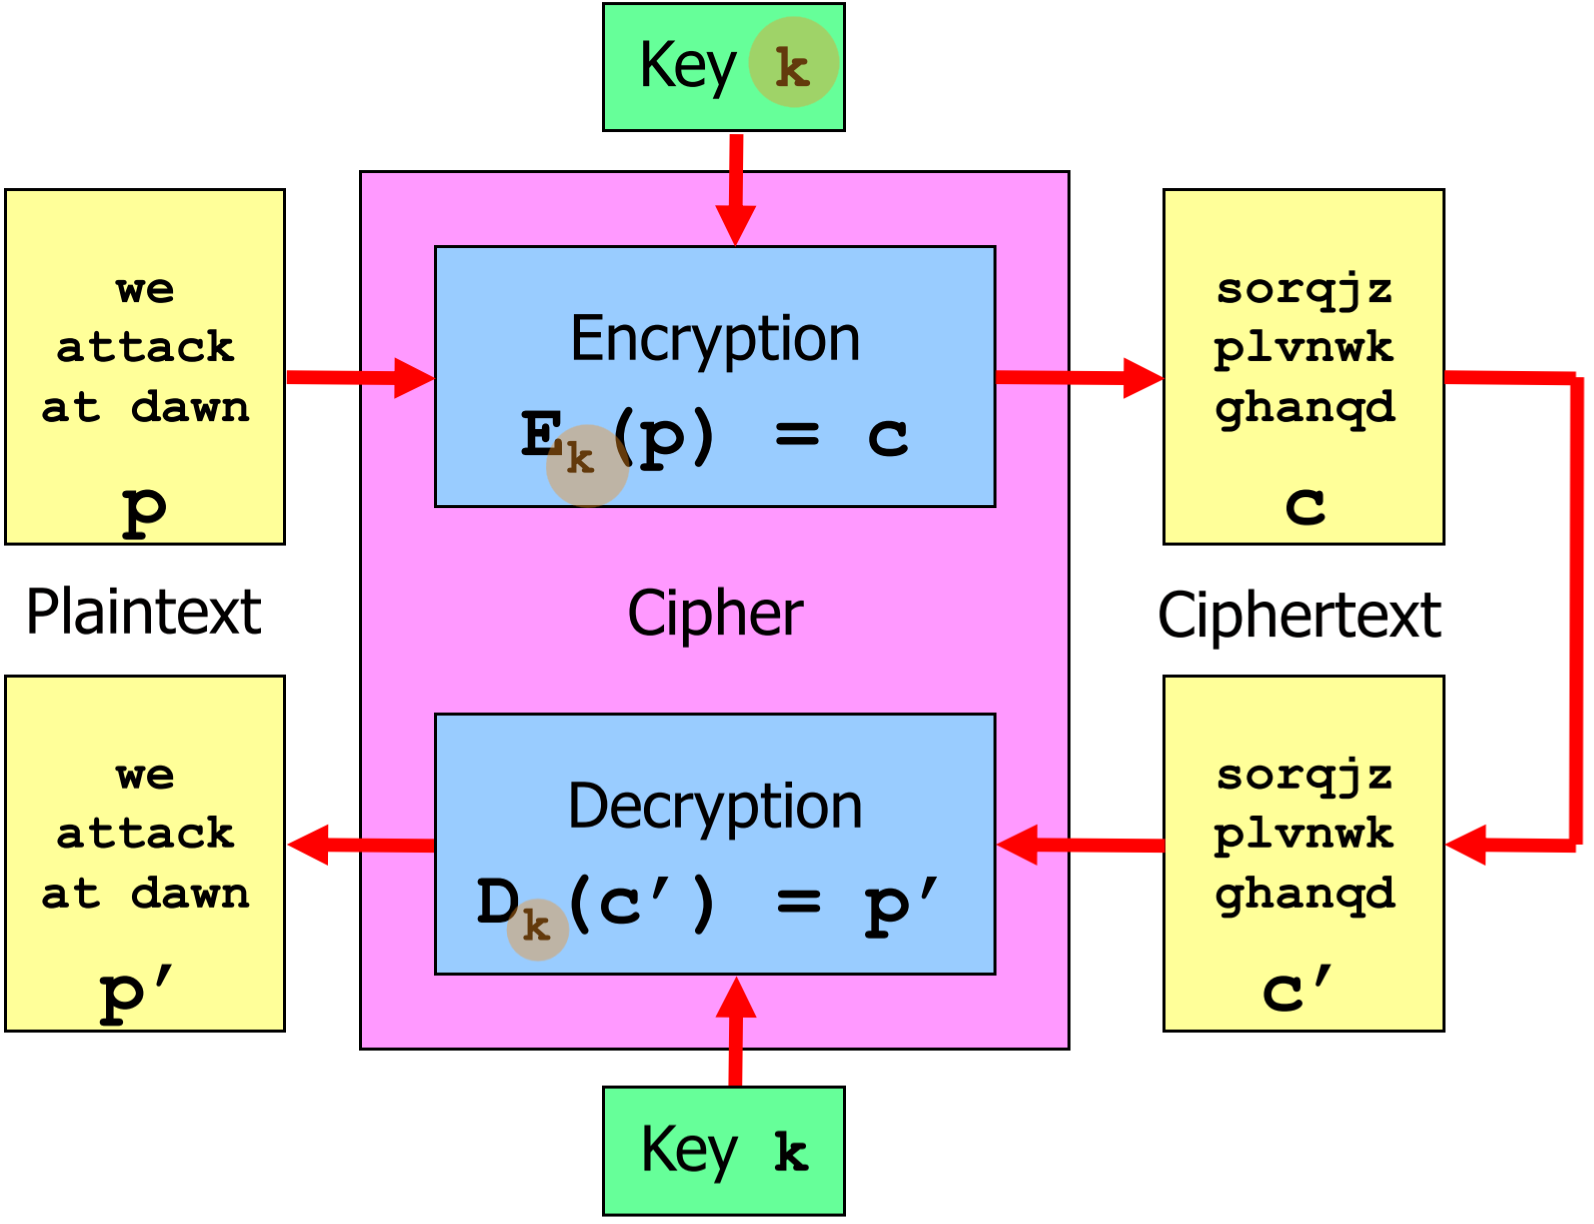
\includegraphics[width=150px]{img/BasicTerminologySecKeyCrypto.png}
%        \captionof{figure}{Basic Terminology basierend auf Secret Key Cryptography}
%        \label{fig:Basic Terminology}
%    \end{Figure}

\chapter{Resulats}

\section{Technical Requirements}
In this section I focus on the technical requirements, which should be considered for the final decision. 

\subsection{Safety and security}
One of the most important requirement is data security. At any time, the data should be stored only encrypted. Every communication with other hospitals or practice should be encrypted. Furthermore, an automatic backup of data is required. 

\subsection{Patient health record}
Since the exchange between the different stakeholders get more complex, it should be possible to manage all data and information electronically. 

\subsection{billing process}
The practice can handle the entire account, especially the entire invoicing/billing process, directly through the system. This allows the practice to handle the entire process more efficiently, which has to be done after the patient’s visit.

\subsection{stock control}
The electronic stock control, helps us to provide a high level on quality. The most important drugs are available at any time, as soon as there are only a few left it sends a message to the physician assistant to restock the drug. 

\subsection{Medication Management}
As soon as the disease is detected, in most cases a medication is prescribed. This prescription should automatically be checked for any conflicts (allergies, other medications etc.) and the general practitioner should be informed.

\subsection{Patient registration}
When a new patient is admitted to the practice, the patient should have the possibility to enter his information (allergies, health insurance etc.) directly via tablet. This relieves the work of the physical assistant.

\subsection{Book online an appointment}
The patient should have the possibility to book an appointment online. The online calendar shows only the available appointments. Once a new appointment is booked, it automatically set the appointment to the general practitioner.

\subsection{Workload}
The physical assistant can directly manage the workload of the general practitioner as well as some other tasks. In this case you have an overview and manage the private practice more efficiently.

\subsection{reports}
Based on all data which are captured it can automatically generate a report of any patient. This report summaries all the relevant information as well as gives a overview about the current disease.

\subsection{statistical reports}
A statistical report of the private practice can be obtained at any time. This allows, for example, an evaluation of the stock management or the workload of the private practice. 

\section{Important standards that should be supported by PIS}
If you want to introduce a new PIS, there are several standards to follow. Of course the PIS has to comply with Swiss law and guidelines. 
An explanation of data protection in medical practices can be found \href{https://www.edoeb.admin.ch/edoeb/de/home/datenschutz/gesundheit/erlaeuterungen-zum-datenschutz-in-der-arztpraxis.html}{here}\\

One of the most important standards is data protection. The so-called \href{https://gdpr-info.eu/}{GDPR}.\\

In addition, there are various standards on how to deal with data transfer and the associated interface (API).
\begin{itemize}
   \item OPAN (Spitex)
   \item EasyNet (Argomed)
   \item DocBox (Visionary)
   \item BlueConnect and BlueEvidence (BlueCare)
\end{itemize}


\section{Top-5 Systems}

\subsection{AESKULAP by Kern Concept AG}
\textbf{Website}: \href{https://kernconcept.ch/aerztesoftware/}{to kernconcept website} \\
\textbf{Price-range}: Available upon request\\ 
\textbf{Standard package}: 
\begin{itemize}
   \item Master data management
   \subitem for patients
   \subitem for treatments
   \subitem for tariffs 
   \item Activity recording and billing
   \subitem with online TARMED-Optimizer and -Validator correspondence
   \item reporting
   \subitem WORD interface with form library 
   \item Medication article management
   \subitem Medication
   \subitem stock management and practice pharmacy
   \item further
   \subitem Statistics
   \subitem dunning 
\end{itemize}

\textbf{Additional modules}:
\begin{itemize}
   \item Laboratory device interface
   \item external laboratory interface
   \item further device integration
   \item digital document archiving directly at the patient's site with the option of archiving in PDF (in separate software)
   \item electronic image archiving directly with the patient integration of imaging medicine 
   \item Devices with connection to the patient
   \item electronic invoicing with the involvement of the usual TrustCenter (TrustX) and with the involvement of MediData AG (MediPort)
   \item electronic media ordering (to wholesaler) also possible with interaction and allergy check at the drug level
   \item integration of X-ray images: digital administration tool with reminder function with patient-based orders after work
   \item e-mail module, SMS module
   \item smart text module
   \item KG macro module
   \item BlueEvidence interface
   \item DocBox communication
   \item text recognition OCR
   \item online practice module
   \item access authorization module
   \item history module
   \item sighting module. 
\end{itemize}


\subsection{CuraMED / curabill by Swisscom}
\textbf{Website}: \href{https://www.swisscom.ch/de/business/enterprise/angebot/e-health/curamed.html}{to the website curaMED}\\
\textbf{Price-range:} available upon request\\

The modern practice software curaMED opens new doors to efficient and effective practice management for doctors and physiotherapists in individual 
practices and outpatient health centers. The Software-as-a-Service (SaaS) solution, configured according to the highest security standards, 
offers a modern and comprehensive medical information system that you can use according to your needs:\\
\textbf{Standard package}:
\begin{itemize}
   \item electronic medical history
   \item practice agenda and resource planning
   \item patient registration (also online via Tablet)
   \item automated service recording
   \item daily journal
   \item statistics and evaluation
   \item search function
\end{itemize}

\textbf{additional module}:\\
wisscom Health takes care of the complete accounting (curabill) on request. Curabill has to paid additionally.


\subsection{MediWin CB by Ärztekasse}
\textbf{Website}: \href{https://www.aerztekasse.ch/angebotsuebersicht/informatik/praxissoftware-mediwin-cb/ }{to the website MediWin}\\
\textbf{Price-range}: Free in the basic version for members of the Ärztekasse. Further modules available upon request/payment 
The medical insurance company provides network-compatible software with powerful instruments. It is suitable for individual and group practices and offers patient management, 
a treatment and session assistant, a medication tool and document management in the free full version. The software can also be expanded with a digital agenda and electronic medical history. \\

\textbf{Standard package} 'All in one Patient administration:
\begin{itemize}
   \item Patient data
   \item Patient cockpit (all relevant data at a glance)
   \item Treatment and session management
   \item Activity recording and billing
\end{itemize}

\subsection{EPaad by Compass IT AG }
\textbf{Website}: \href{https://epaad.ch/}{to the website EPaad}\\
\textbf{Price-range}:CHF 7000 for the practice and the first user, afterwards CHF 3500 for every additional user. \\
\textit{Alternatively}: CHF 2000 per year and CHF 1000 for every other user per year \\
\textbf{Standard Package:}
\begin{itemize}
   \item Clearly arranged patient administration with complete ECG
   \item simple appointment management
   \item handling at reception
   \item recording of treatment
   \item billing of treatments
   \item administration of master data
   \item integrated ordering system (medication/material)
   \item statistics 
\end{itemize}

\textbf{Additional modules}: 
\begin{itemize}
   \item Software as a Service (SaaS) in the practice/cloud possible
   \item mTAN
   \item replication on backup server out of practice
   \item access over several locations
   \item tablet version inclusive daily update of service providers and medications
   \item data import/export
   \item patient comparison via insurance card or tel.search
   \item document storage at the patient's location
   \item printing of labels/appointment cards
   \item dispatch of all documents (transfer, report, etc.) via mail
   \item history documentation
   \item generation of reports (blocks can be taken over from SOAP)
   \item list of pending items
   \item internal/external laboratory equipment interface with automatic import
   \item laboratory order
   \item digital X-ray images at the patient's or via PACS
   \item medical equipment integration via GDT
   \item image management Dicom
   \item electronic invoicing (Trust Center, MediData, health insurance company etc.)
   \item automatic ordering of medication and material
   \item recall function with reminder to phone, SMS or mail
   \item appointment wizard
   \item appointment booking option for the patient
   \item resource management
   \item service blocks
   \item favorites
   \item debtor control/monitoring
   \item Tarmed validation 
\end{itemize}


\section{Best practice for the evaluation of IT Systems}
There are various procedures for evaluating an IT system. Personally, I would recommend that you use a proven approach. 
Basically I refer to \textit{\href{https://www.fmhservices.ch/softwarekatalog}{FMH Software Overview}}. 
FMH not only offers a good overview of the individual providers, but also provides step-by-step instructions for the evaluation of a PIS.
\begin{enumerate}
   \item Vision, digital strategy, goal
   \item Requirements
   \item Evaluation and offer
   \item Contract and Project management
   \item Project approval and daily business
\end{enumerate}

In addition, I have included other helpful links for the evaluation. 
\begin{itemize}
   \item \href{https://gaeso.ch/partnernews/harte-fakten-sachen-praxissoftware }{possible guideline}
   \item \href{https://www.gryps.ch/produkte/praxissoftware-196/?gclid=EAIaIQobChMI05zh7t7t6wIViN4YCh11fwA3EAAYAyAAEgLCTfD_BwE}{PIS Software-Evaluation}
   \item \href{https://www.gryps.ch/produkte/praxissoftware-196/praxissoftware-kosten/}{PIS costs and factors}
\end{itemize}


\end{document}